\documentclass[12pt,letterpaper]{article}
\usepackage[utf8]{inputenc}
\usepackage[spanish]{babel}
\usepackage{amsmath}
\usepackage{amsfonts}
\usepackage{amssymb}
\usepackage{graphicx}
\usepackage[left=2cm,right=2cm,top=2cm,bottom=2cm]{geometry}
\author{Oscar Daniel Rosario Morales,Israel Hipolito Mejia 
Alba}

\title{Practica N 12 " ALGORITMOS PARALELOS 1" 
EDA 2}
\begin{document}
\maketitle
Grupo: 8 


Profesor : Tista Garcia Edgar

\newpage
\subsection{Objetivo:}
El estudiante conocerá y aprenderá a utilizar algunas de las directivas de OpenMP para implementar algún algoritmo paralelo.

\subsection{Actividades:}
-Realizar ejemplos de funcionamiento de directivas de OpenMP en el lenguaje C, tales como los constructores critical, section,single,master,barrier y las cláusulas reduction y nowait.
-Realizar programas que resuelvan un problema de forma paralela utilizando distintas directivas de OpenMP.
\subsection{Desarrollo}
\subsubsection*{Actividad 1 Completar la versión serie y paralela del ejemplo explicado de búsqueda del valor mayor de los elementos de un arreglo unidimensional de enteros}
\textbf{Algoritmo secuencial.}

Podemos ver como el algoritmo busca elemento a elemento el de mayor valor y lo va guardando en la variable max si este cambia, para al final solo imprimirlo.

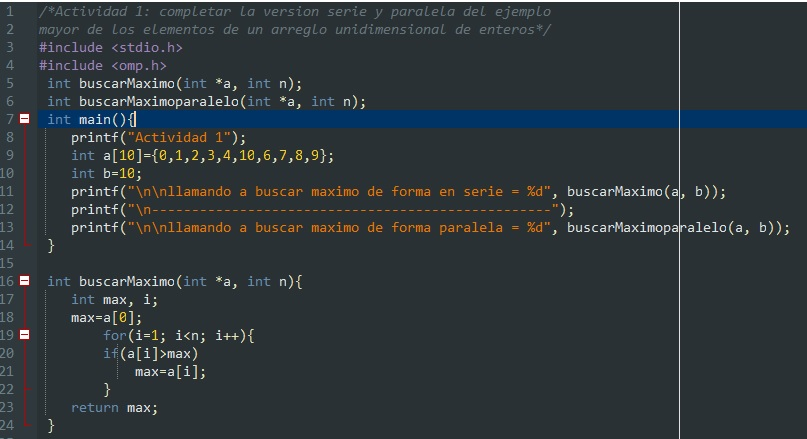
\includegraphics[scale=.8]{12-1-1.jpg} 
\textbf{Algoritmo paralelo.}

Este algoritmo las iteraciones del ciclo for en distintos hilos con parallel for, después con la directiva critical hace que se use la variable max un hilo a la vez para no tener problemas al actualizar su valor en ejecución.

\subsubsection*{Actividad 2 . Completar la versión serie y sus dos versiones paralelas del ejemoki explicado del producto punto de dos vectores de n elementos enteros}
Tuvimos problemas al mandar a llamar las funciones y a pesar de estar revisándolas constantemente, no logramos hacer que funcionaran, sin embargo realizamos esta actividad nuevamente pero sin usar métodos y logro funcionar. Primero  se mostrara el intentento fallido y después el que si funciona.
A continuación se muestran capturas de panrallas del primer intento:

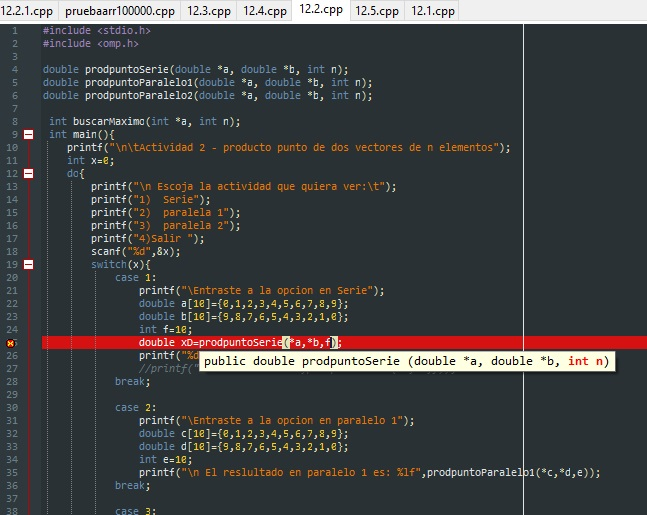
\includegraphics[scale=.8]{13.jpg}

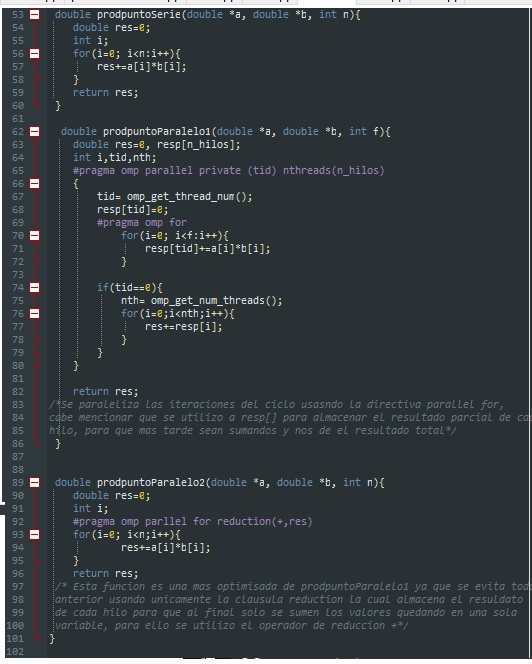
\includegraphics[scale=.8]{14.jpg}

 Si el programa hubiera funcionado, en la función prodpuntoSerie se ubiera hecho la suma de todos los resultados de la multiplicación de cada elemento de ambos arreglos en un solo hilo, por lo que se haría el producto punto como normalmente se conoce.
En  el primer producto punto paralelo, se usaría parallel for para realizar la paralelización de las iteraciones de cada ciclo y con resp[] se almacena cada resultado parcial de cada hilo, de esta manera al final solo se suman y tenemos nuestro producto punto realizado en conjunto de todos los hilos.
Finalmente con el prodpuntoParalelo2  se utiliza únicamente la cláusula reduction(+,res) lo cual nos suma todos los resultados de res en cada hilo, de tal manera que al final tenemos un único valor para res, que es el que retorna. 
Ahora analizaremos rápidamente el segundo intento en el que si funciono correctamente:

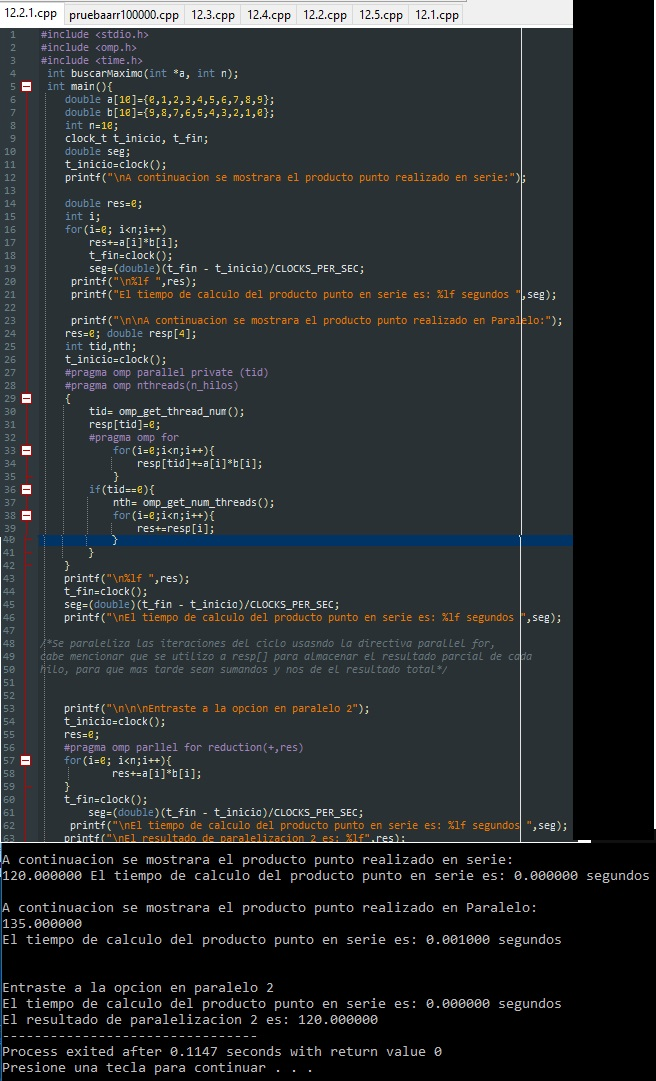
\includegraphics[scale=.8]{15.jpg}

Se puede ver que para este caso tuvimos que usar parallel private  y ntdreads de manera separada para que funcionara el programa en el caso de paralelo 1, además se hizo uso de la librería time.h para medir el tiempo, fuera de eso el procedimiento es mismo, solo que ya no usamos funciones para que el programa haga cada acción.


\subsubsection*{Actividad 3 Obtención del numero Pi utilizando la regla del trapecio}
Para esta actividad se realizó la parte secuencial con el código dado en la práctica y se hizo paralelo poniéndole un parallel for  antes del ciclo que le da valor a x y en consola podemos ver la siguiente información: 

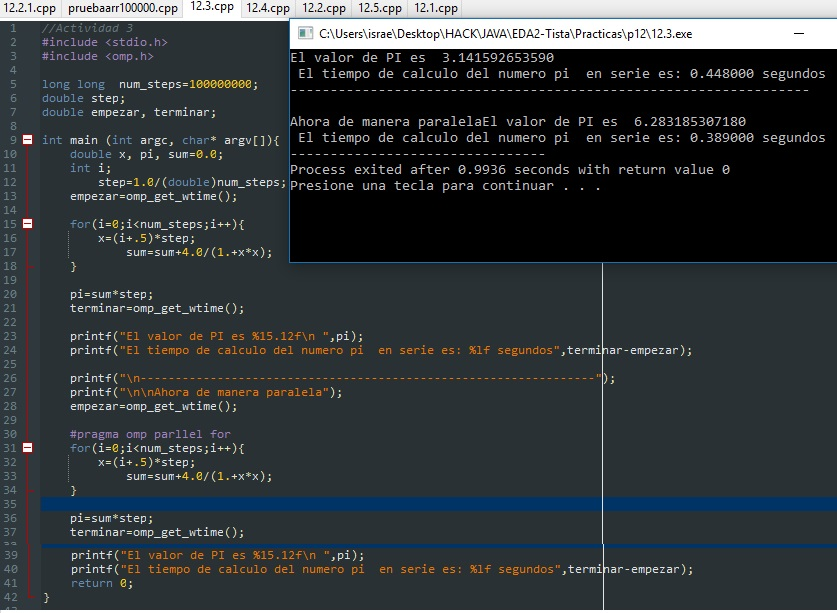
\includegraphics[scale=.8]{16.jpg}

\subsubsection*{Actividad 4 Obtencion del resultado usando el constructor for y  section}
Esta actividad no se pude realizar del todo ya que al usar el contructor for esperábamos que se realizara las iteraciones de los ciclos for de manera paralela, pero los resultados se desborraban. Por otro lado al usar el constructor sections se esperaría que cada ciclo se realizara de manera independiente por hilo, sin embargo, no estamos del todo seguros que fue así y después de esto la salida a pantalla nos da a entender que retorna el resultado aunque no se pidió que lo hiciera de esta manera.

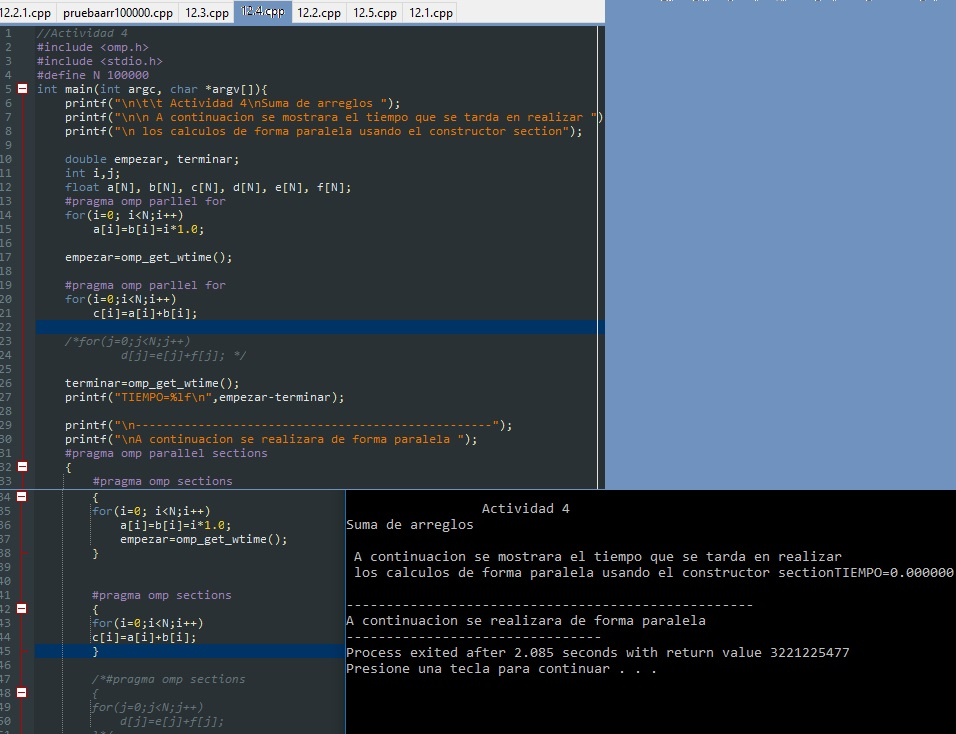
\includegraphics[scale=.8]{17.jpg}

\subsubsection*{Actividad 5}
¿Qué sucede si se quita la barrera? Los hilos realizan sus operaciones sin esperar que el hilo maestro acabe de imprimir los elementos del arreglo

Si en lugar de utilizar el constructor master se utilizara single, ¿Qué otros cambios se tienen que hacer en el cogido? Estuvimos checando si era necesario realizar algún cambio, pero no lo encontramos, al parecer el programa funciona correctamente como se ve en la imagen. Cabe destacar que al hacer uso del constructor single todos los hilos tienen que esperar a que termine de imprimir este hilo.

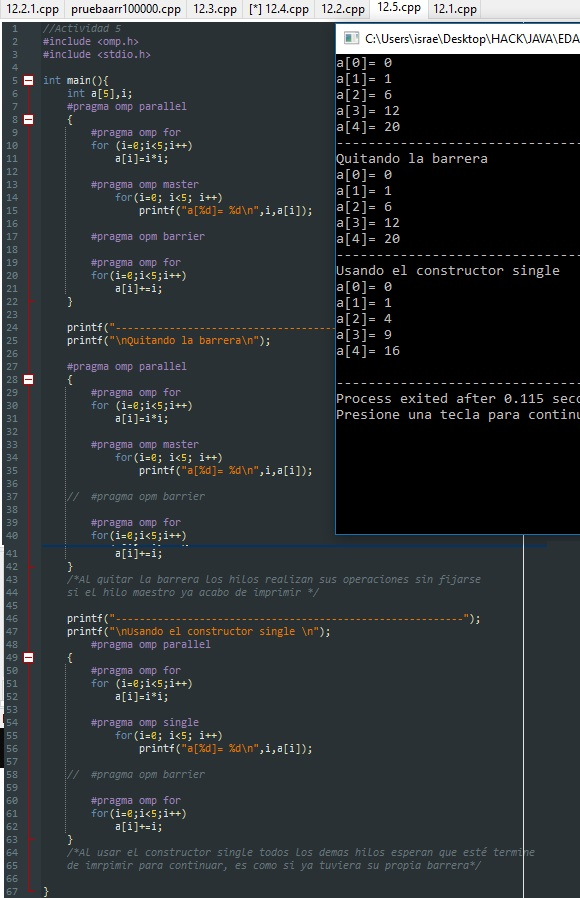
\includegraphics[scale=.8]{18.jpg}
\newpage

\section{Conclusiones}

\subsubsection*{Rosario Morales Oscar Daniel }
En la realización de está practica se pudo comprender de manera teórica distintas directivas de OpenMp, como lo fue section, master y sus relaciones con las barreras. A pesar de que ya habíamos realizado la practica 13 porque pensamos que esa será más complicada, no logramos realizar esta como se esperaba, pero considero que los conocimientos los pudimos obtener fueron buenos y sirvió para ver de otra manera distintos aspectos que logramos hacer en la practica 13.

\subsubsection*{Israel Hipolito Mejia 
Alba}
La realización de esta práctica fue un tanto extraña, ya que primero hicimos la 13 pensando que nos tardaríamos más en ella, pero después cuando intentábamos hacer esta nuestros programas marcaban múltiples errores y a pesar de que comprendíamos la parte teórica de la guía de laboratorio, cuando lo queríamos pasar a código se nos complicó mucho y en algunos casos no funcionaba correctamente. De cualquier manera, sirvió para reforzar, aunque sea un poco más nuestros conocimientos, como algo completamente nuevo para mi fue la cláusula reduction.



















\end{document}
